\documentclass[11pt,a4paper]{article} % Сурс - семинары по алгебре Медведя Никиты Юрьевича
\usepackage[utf8]{inputenc}
\usepackage[T2A]{fontenc}

\usepackage[english,russian]{babel}
\usepackage{amsfonts,amssymb}
\usepackage{graphicx}
\graphicspath{ {.} }

\usepackage{amsmath}
\usepackage{amsthm}
\usepackage{relsize}

\usepackage{systeme}

\usepackage{indentfirst} % Красная строка
\usepackage{fancyhdr}
\usepackage{wrapfig}
\usepackage{textcomp}

\usepackage{xcolor}% http://ctan.org/pkg/xcolor
%\usepackage{colortbl}% http://ctan.org/pkg/colortbl
\usepackage{multirow}% http://ctan.org/pkg/multirow
\usepackage{graphicx}% http://ctan.org/pkg/graphicx

\usepackage[unicode]{hyperref}

\usepackage{scontents}

% Blank formula checking
\usepackage{ifthen}
\newlength{\pheight}

\usepackage{centernot}
\usepackage{tabularx}
\usepackage{adjustbox, array, hhline}
\usepackage{makecell}

\addtolength{\textwidth}{120pt}
\addtolength{\hoffset}{-3cm}
\addtolength{\voffset}{-3cm}
\addtolength{\textheight}{170pt}

\tolerance=3000
% \flushbottom

\parindent=1cm

\begin{document}

\hspace{-1cm} 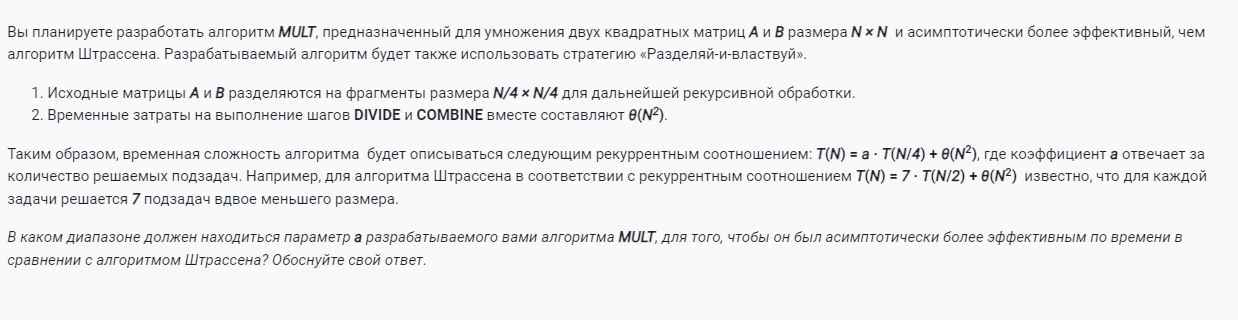
\includegraphics[scale=0.60]{a3_df.png}

\begin{tabular}{l}
    1. Найдём асимптотическую точную оценку для функции временной сложности \\
    алгоритма Штрассена: \\
    $ T(N) = 7 \cdot T\left(\frac{N}{2}\right) + \Theta(N^2) $ \\
    Обозначим $ a = 7, b = 2, c = 2 $, тогда $ T(N) = a \cdot T\left(\frac{N}{b}\right) + \Theta(N^c) $ \\
    $ a, b \text{ и } c $ не зависят от $ N \implies $ можно применить master-теорему \\
    $ c = 2 = \log_2 4 < \log_2 7 = \log_b a \implies $ по второй формулировке master-теоремы \\ 
    $ T(N) = \Theta(N^{\log_b a}) = \Theta(N^{\log_2 7}) $ \\
    \\
    $ 2. \text{ Для алгоритма MULT } T(n) = a * T(\frac{n}{4}) + \Theta(n^2) $ \\
    $ a $ - количество решаемых подзадач $ \implies a \in \mathbb{N}$ \\
    Для данного алгоритма $ b = 4, c = 2. $ Они не зависят от $ N \implies $ можно применить master-теорему \\
    $ c = 2 = \log_4 16 $ \\
    $ \log_b a = \log_4 a $ \\
    \begin{tabular}{l}
        \\
        $ I. $ $ a > 16 \implies \log_b a > c \implies \text{по master-теореме } T(N) = \Theta(N^{\log_b a}) =\Theta(N^{\log_4 a}) $ \\
        Чтобы алгоритм MULT был асимптотически более эффективным в сравнении с \\
        алгоритмом Штрассена, необходимо, чтобы начиная с какого-то номера выполнялось неравенство \\
        $ N^{\log_2 7} > N^{\log_4 a} \iff \log_2 7 > \log_4 a \iff 49 > a $ \\
        \\
        $ II. $ $ a = 16 \implies \log_b a = c \implies \text{по master-теореме } T(N) = \Theta(N^c \log N) = \Theta(N^2 \log N) $ \\
        Чтобы алгоритм MULT был асимптотически более эффективным в сравнении с \\
        алгоритмом Штрассена, необходимо, чтобы с какого-то номера выполнялось неравенство \\
        $ N^{\log_2 7} > N^2 \log_q N \iff N^{\log_2 1.75} > \log_q N $, где $ q > 0 \wedge q \ne 1 $ \\
        $ \log_2 1.75 > 0 \implies \forall q ((q > 0 \wedge q \ne 1) \implies \exists N_0 \in \mathbb{N} \hspace*{2pt} \forall N \ge N_0: N^{\log_2 1.75} > \log_q N) $ \\
        (менее формально, показательная функция с любым показателем > 0 и основанием N > 1 \\
        растёт быстрее, чем логарифм от N по любому основанию) \\
        \\
        $ III. $ $ a < 16 \implies \log_b a < c \implies \text{по master-теореме } T(N) = \Theta(N^c) = \Theta(N^2) $ \\
        $ c = 2 = \log_2 4 < \log_2 7 \implies N^c < N^{\log_2 7} \implies \text{ при } a < 16 $ алгоритм MULT \\
        всегда асимптотически более эффективен в сравнении с алгоритмом Штрассена
        
    \end{tabular}
    \\
    \\
    Ответ: $ a \in [1; 48] \cap \mathbb{N} $
\end{tabular}
\end{document}
